\documentclass{sig-alternate}
\usepackage{graphicx, url}

\newcommand{\strong}[1] {\textbf{#1}}
\newcommand{\code}[1] {\texttt{#1}}

\begin{document}
\title{Text Sliding: Information Discovery with Intensely Integrated Text Analysis}
\numberofauthors{4}

\author{% 1st. author
\alignauthor Firstname LastName\\
       \affaddr{Address}\\
       \affaddr{Address}\\
       \affaddr{Address}\\
       \email{email@address.edu}
% 2nd. author
\alignauthor Firstname LastName\\
       \affaddr{Address}\\
       \affaddr{Address}\\
       \affaddr{Address}\\
       \email{email@address.edu}
% 3rd. author
\alignauthor Firstname LastName\\
       \affaddr{Address}\\
       \affaddr{Address}\\
       \affaddr{Address}\\
       \email{email@address.edu}
% 4th. author
\and
\alignauthor Firstname LastName\\
       \affaddr{Address}\\
       \affaddr{Address}\\
       \affaddr{Address}\\
       \email{email@address.edu}
}

\maketitle

\begin{abstract}
There are numerous information analysis and discovery tools that allow users to view multidimensional data from different angles by selecting subsets of data, viewing those as visualizations, moving laterally to view other subsets of data, slicing into another view, expanding the viewed data by relaxing constraints, and so on.  However, these tools operate over numerical and categorical data, but do not seamlessly operate over raw textual information with the same flexibility. In this paper we describe a text analysis and discovery tool that allows for highly flexible  ``slicing and dicing'' (hence  ``sliding'') across a text collection.  The goal of the tool is to help scholars and analysts discover patterns and formulate and test hypotheses about the contents of their text collections, midway between what traditional humanities scholars call a  ``close read'' and the digital humanities  ``distant read'' or "culturomics" approach.  We illustrate the text sliding capabilities of the tool with two real-world case studies from the humanities and social sciences -- the practice of literacy education, and U.S. perceptions of China and Japan over the last 30 years -- showing how the tool has enabled scholars with no technical background to make new, important discoveries in these text collections.

\end{abstract}

% A category with the (minimum) three required fields
\category{H.X}{XXXXX XXXXXXX XXXX}{XXXXX}

%A category including the fourth, optional field follows...
\category{H.X}{XXXXX }{XXXXX }[XXXXX ]

\keywords{exploratory data analysis, text mining, information visualization, digital humanities}

\section{Introduction}
Current text analysis systems put computational linguistics and data visualization into the hands of users. Tools such as Jigsaw, IBM TextMiner, and SAS Text Analytics take techniques like text classification, named-entity recognition, sentiment analysis and summarization and build systems to automate their use. To make the results of these computational analyses interpretable, they display the outputs with interactive data visualization. These systems have made advanced text mining and visualization algorithms available to users without expertise in those areas.

However, language is a unique form of expression, and text as data is distinct from numerical and categorical data.  Text has both linear and hierarchical structure, its meaning is ambiguous given its representation, it has tens of thousands or hundreds of thousands of features, and frequencies of words are distributed via a power law.  
 Even a small fragment of text does not stand alone, but is densely interconnected with other text through the \emph{linguistic phenomena} that it contains. These are units of meaning that take surface form in text, such as words, phrases, relations between words (including synonymy and hyponymy) and literary devices, such as metaphor, sarcasm and allusion. To illustrate, consider this 13-word ``slice'' of text from Shakespeare's ``Romeo and Juliet", where a slice is simply a set of sentences (not necessarily consecutive, like in this example):

\begin{verbatim}
ROMEO:
    Is she a Capulet?
    O dear account! my life is my foe's debt.
\end{verbatim}

Surrounding this tiny slice is a swarm of other slices of text, each associated with the different linguistic phenomena in this slice. For instance:
\begin{itemize}
\item Each of the 11 distinct words in the above excerpt can be thought of as a jumping-off point to all of the other sentences in which it occurs, as well as to sentences containing other words that mean the same thing, or to other words that tend to be used near it.
\item Each  two-, three-, or n-word phrase can be associated with every other sentence in which it occurs
\item  Each grammatical relationship between words (such as ``dear" being an adjective modifier of  ``account") can be thought of as a link to other words that enter that relation (other adjectives describing ``account", or other things that are ``dear".)
\item Each instance of a literary device, such as the exclamation ``dear account'', or the imagery of debt, can be associated with all other occurrences of this phrase, or the different phrasings with which this concept surfaces in the play.
\end{itemize}

The more structure there is to text, the more kinds of associations are possible. Shakespeare plays have metadata, such as speaker, act, and scene, so associations based on these dimensions also exist:
\begin{itemize}
\item The speaker, Romeo, can be associated with all the other speeches by him.
\item The location within the play: Act 1, Scene 4 can be associated with the other scenes in that act, or the other speakers in that scene.
\end{itemize}

This network of associated slices is immediately apparent to us as humans. And to an analyst trying to make sense of an idea, some associations may be extremely meaningful. In fact, transitions  and associations are central to the analytical process. People seeking knowledge from text are engaging in \emph{sensemaking}. They do not follow a straight path from data input to analysis output, but meander between analysis, interpretation, exploration and understanding on different sub-collections of data.  It is therefore important for text analysis systems to support not just algorithmic and visual analysis, but the transitions: slicing, filtering and exploration that lead from analysis to analysis, visualization to visualization, and finally to insight.

In this paper, we describe a text analysis tool that supports such transitions. It allows highly flexible slicing and dicing, as well as frictionless transitions (hence ``sliding") between visual analyses, drill-downs, lateral explorations and overviews of slices in a text collection. Our tool uses computational linguistics, information retrieval and data visualization, and enables scholars with no technical background to conduct analyses yielding concrete, useful and otherwise inaccessible knowledge.

\subsection{Humanities and Social Sciences}
The humanities and social sciences (HASS) are our motivation. In these fields, it is common for scholars to have hundreds, even thousands of text-based source documents of interest from which they extract evidence for complex arguments about society and culture. These collections (such as the set of all New York Times editorials about China, the complete works of Shakespeare, or the set of all 18th C. American novels)  are difficult to make sense of and navigate. Unlike numerical data, they cannot be condensed, overviewed, and summarized in an automated fashion without losing significant information. And the metadata that accompanies the documents -- often from library records -- does not capture the varied content of the of the text within.

HASS scholars are an important area of focus for tool builders for another reason: low uptake. A 2012 study of computational tool use among these scholars showed that adoption was low despite an abundance of tools. The main culprit? Poor interface design due to lack of involvement with end users. In our research, we have tried to avoid this problem by taking an iterative, user-centered design approach. We collaborate with active HASS scholars working on text analysis problems of existing professional interest to them, and let their needs, behaviors, and observations drive tool development.

We introduce the text sliding capabilities of our tool using two case studies. The researchers driving these studies used our tool to further their projects on  education and U.S-China relations. The two projects investigated
\begin{enumerate}
	\item How college students from diverse backgrounds remember and reflect upon literacy.
	\item How U.S. perceptions China and Japan responded to China's rise over the last 30 years.
\end{enumerate}

This paper is structured as follows: in the next section, we describe results from the field of sensemaking that motivate the need for ``sliding'' interactions between slices. After that, we explain the main ideas behind text sliding and show it in action with extended examples from case studies. Then, we describe related systems, and finally conclude with a discussion our results and future work.

\section{Motivation}
Observational studies from the literature on sensemaking describe many problems analysts encounter while trying to make sense of text collections. These studies typically watch professionals such as government intelligence analysts \cite{x}, business analysts \cite{x} market researchers \cite{x} and academics \cite{x} at work, attempt to categorize the actions they perform and identify common sequences of actions. Several models of the sensemaking process have emerged \cite{x} These models attempt to explain what one would observe when watching analysts distill understanding from raw data, where ``understanding" usually manifests itself as a summary, report, or presentation.

Pirolli and Card \cite{pirolli_sensemaking_2005} identified ``pain points" in three areas having to do with navigation and transitions between slices while studying intelligence analysts working with large collections of text-based reports:
\begin{enumerate}
\item \strong{Exploring} the collection by searching and filtering. Collections were often large difficult to navigate. 
	\begin{itemize}
		\item If  associated slices were easy to see and to access, exploration might become easier. 
	\end{itemize}
\item \strong{Enriching}, which is the process of collecting a narrower set of items for analysis. This was a time consuming process involving going through documents returned by results, reading them to determine whether they were relevant or not, and placing them into groups.
	\begin{itemize}
		\item It should be easy to select documents matching a term, quickly skim the text to determine relevance, and to collect the relevant text into a slice for later analysis.
	\end{itemize}
\item \strong{Exploiting}, which is the process of analyzing the collected information by manual schematizing, computational analysis, or visualization. Follow-up actions, such as drilling down to a finer set, noticing something interesting and starting a different analysis, or re-framing the question had a high cost.
	\begin{itemize}
		\item It should be easy to explore associations and to start new threads of inquiry with low overhead, and without losing their current state.
	\end{itemize}
\end{enumerate}


\section{Text Sliding}

The twin concepts of \emph{slices} and \emph{views} are central to text sliding. A slice is a set of sentences, and a view is a visual representation of the data in a slice: anything from a list of the sentences in the slice, to more complex linguistic processing combined with visual analytics.  A slice is like a scientific specimen, a sample of some chemical compound. and views are the different lenses, apparatuses, and tests that reveal different information about the sample.

Through the richness of language, slices are \emph{linguistically associated} with other slices (that also contain a particular word or phrase for example). If there is metadata accompanying the text, such as Act, Scene, and Speaker in Shakespeare's plays, there are also \emph{metadata associations}. Finally,  through the wide variety of visual analytics tool available, there can be many different ways of viewing and analyzing the data in a single slice. Text sliding makes all these associations accessible. 
 In fact, we define text sliding as:
\begin{itemize}
	\item Getting a different view of the same slice (lateral movement)
	\item Opening a new view of an associated slice (drilling down, following a new thread, or `more like this')
\end{itemize}

\subsection{Slices}
In our tool, we define a slice as \emph{a set of sentences}, although future tools might use different units of text, such as paragraphs, documents, or phrases. We allow arbitrarily-assembled slices, but it is easiest to think of slices as combinations of searches and filters. 

Slices are conceptually illustrated in Figure \ref{fig:slices}. In that figure, we are assembling a slice corresponding to all sentences spoken by Romeo  in Act 1 in which he mentions ``Capulet''. We start with the whole collection, the collected works of Shakespeare, apply filters for \code{speaker = Romeo} and \code{act = Act 1}  and and also apply a search for \code{`Capulet'}. This leaves us with a slice containing only sentences that match our criteria, in this case, only one sentence:
\begin{verbatim}
 	{`Is she a Capulet?'}
\end{verbatim}

\subsubsection{Linguistic Associations}
Slices do not stand alone. In our database, each sentence is indexed according to the following linguistic phenomena:
\begin{itemize}
  \item Each word in the sentence, and its part of speech (noun, verb, adjective, etc.)
  \item Each consecutive two-, three-, and four-word sequence in the sentence
  \item Each grammatical relationship in the sentence. (These are identified using a computational linguistics technology called dependency parsing, fully explained in \cite{jurafsky_chapter_2009}. In particular, we use the Stanford dependency parser\footnote{Online demo  at \url{http://nlp.stanford.edu:8080/parser/}}\cite{klein_accurate_2003}.
\end{itemize}
By traversing these index both ways, we can quickly compute the associations for a slice. From a slice, we can query for all the words, phrases, or grammatical relations in the sentences in that slice, and from there, to all the other sentences that contain each particular item.

Figure \ref{fig:slices-associated} illustrates the other slices associated with the slice from figure \ref{fig:slices}. That slice only contains one sentence, \code{`Is she a Capulet?'}, but in our tool, it is associated with the following other slices through the words \code{`is'}, \code{`she'}, \code{`a'} and \code{`capulet'}, grammatical relationships between those three words and other words in the collection, and the phrases \code{`Is she'}, \code{`she a'}, \code{`a capulet'},  \code{`is she a'}, and so on.


\subsection{Views}
\begin{figure}
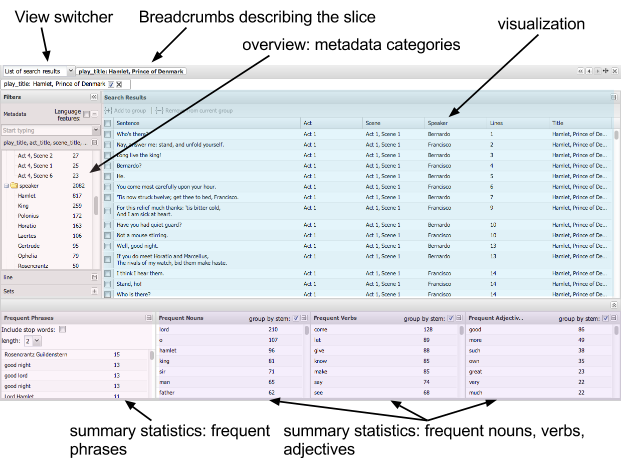
\includegraphics[width=0.5\textwidth]{fig/sliding/01-view-breakdown.png}
\caption{The different components of a view \label{fig:view-schematic}}
\end{figure}
Views are visual representations of a slice. As shown in Figure \ref{fig:view-schematic},  views  are window-like panels, and they contain the following components:
\begin{itemize}
	\item A drop down menu to switch to a different view of the same slice (see Figure \ref{fig:chris03})
	\item Breadcrumbs identifying the slice
	\item A visualization of the data in the slice. Currently, the choices are:
		\begin{itemize}
			\item A list of sentences
			\item A list of documents that match the sentences in the slice
			\item An interactive word tree \cite{wattenberg_word_2008} of the most common word in the slice, or the search term, if specified
			\item Charts of how many sentences in the slice are distributed across various metadata categories
			\item If the slice is a full document, a simple reading interface
			\item If the slice is the result of a grammatical relation query, bar charts showing how often different words in the slice that appear in the relations
		\end{itemize}
	\item Summary statistics of:
		\begin{itemize}
			\item How many sentences within the slice match different metadata categories
			\item The most frequent nouns, verbs, adjectives and multi-word phrases
		\end{itemize}
\end{itemize}

\subsection{Text-Sliding Interactions}

Our goal is to make as many different types of associations and views available without overwhelming the user.
\subsubsection{Lateral Movement}
The easiest slide in our tool is \emph{lateral movement}: creating a different view of the same slice.  There is a drop-down menu at the top left corner of each view which provides this function (Figure \ref{fig:chris03}).  Selecting a different view from the menu opens up that new view (on the same slice) alongside the current one. Users can have as many views open as they want, but most displays get crowded after 2 or 3.  
\begin{figure}[h!]
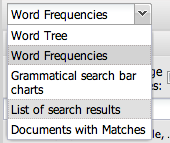
\includegraphics[width=0.2\textwidth]{fig/chris/03.png}
\caption{ This is the view-switcher drop-down menu. It can be found at the top left corner of every view. Selecting an option opens a new view  of the same slice alongside the current view. \label{fig:chris03}}
\end{figure}

\subsubsection{Filtering by Metadata}
On the other hand, interactions for getting to different slices are different depending on the type of association. First, there are simple filters, such as going from \emph{Hamlet} to just \emph{Act 1 of Hamlet}. And simple searches, such as going from \emph{Hamlet} to \emph{sentences containing `good' in Hamlet}.
  
\begin{figure}
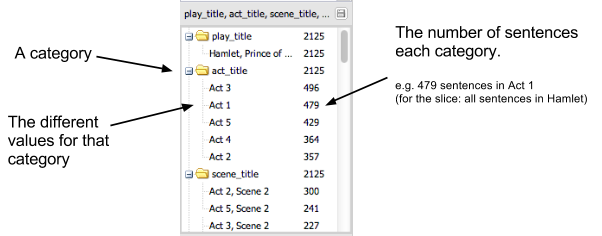
\includegraphics[width=0.5\textwidth]{fig/sliding/02-metadata-categories.png}
\caption{The metadata overview for the slice \code{play = Hamlet}.  It shows how many sentences match different metadata categories. Here, we see that in Hamlet, Act 3 has the most sentences, followed by Acts, 1, 5, 4, and 2. \label{fig:metadata-categories}}
\end{figure}
For filtering a slice by metadata, we use the metadata overview, shown in Figure \ref{fig:metadata-categories}. It is an `overview' in the sense that it shows how many sentences in the slice match each available metadata category, but it is also a filter. Clicking on any particular value creates a new, smaller slice restricted only to sentences that match that value. For example, If we were viewing a list of sentences from Hamlet,  clicking on Act 1 would change the view to just the list of sentences in \emph{Act 1} of Hamlet.

\subsubsection{Restricting to Matches from a Search}


\subsubsection{Overview/Filters by Common Words and Phrases }


\subsubsection{Related Words}

\subsubsection{Grammatical Relationships}

\subsubsection {Creating Arbitrary Sets}

\section{Case Studies}

\subsection{Literacy Autobiographies}

\subsubsection{Introduction}
As a college English Composition instructor,  [FirstName] Ganding, at  [university's] school of Education asks students to write often and in a variety of situations. In this project, he examined ways in which he might draw upon our tool to assist in the teaching and learning of writing. He was particularly interested in the literacy autobiography. In this type of writing, students describe significant experiences they have had with literacy and reflect upon the importance of literacy to their lives.  

He analyzed the content of approximately 140 literacy autobiographies written by students from courses that he has taught over that past two years, each about 1,500 to 2,000 words long. He is familiar with the collection, having previously read and commented on each of the 140 essays included.  Table \ref{table:rex-courses} shows the different courses from which literacy autobiographies were analyzed. The courses were at different colleges and taught at different proficiency levels.

Among the questions that guided his inquiry were the following. In this example, we show how our tool helped him get answers:
\begin{enumerate}
\item What can a distant reading of student literacy autobiographies tell him about students that close readings cannot?
\item What patterns exist in student literacy autobiographies at different course levels and institutions?
\end{enumerate}


\begin{table}
\begin{tabular}{lll}
Course& College & Level \\
\hline
Engl 1A (n=29) & Berkeley City C.& First-year \\
Engl 201AB (n=28) & C. of Alameda & Pre-transfer \\
Engl 5 (n=40) & Berkeley City C. & Transfer level \\
Edu 140 (n=40) & UC Berkeley & Upper division \\
\end{tabular}
\caption{The four different courses, each at a different proficiency level, from which literacy autobiographies were analyzed. \label{table:rex-courses}}
\end{table}


 \subsubsection{A new take on students' experiences}

\begin{figure*}
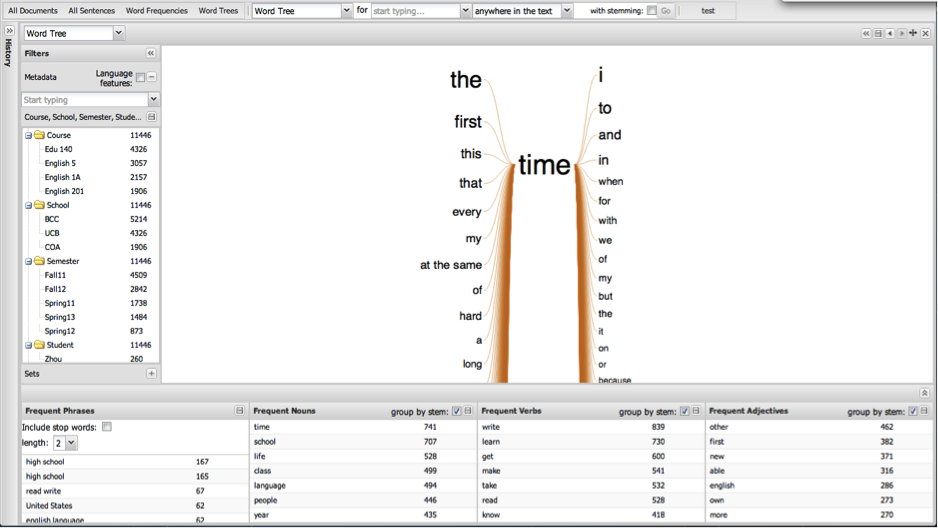
\includegraphics[width=\textwidth]{fig/rex/01.png}
\caption{The initial display when opening the tool \label{fig:rex01}}
\end{figure*}

Ganding don't usually consider the frequencies of words unless a student repeats one to the point of distraction. However, our tool's very first overview (Figure \ref{fig:rex01}) prompted him to consider the significance of individual words and their repeated use:
\begin{quote}
From the moment I opened [the tool], `distance' immediately provided new insight and areas of exploration as I was intrigued by unexpected high word frequencies.  The most obvious example is the frequent use of the word ``time" which is not only the most frequent noun but also the most frequent word overall.  As opposed to ``literacy'', ``language'', and any noun or verb forms of ``read'' and ``write'', the word tree for ``time'' appears before any term is placed in the key word search.   I found similar surprises in the adjective and verb frequencies, and these surprises would guide my decision-making and analysis.
\end{quote}

\begin{figure}
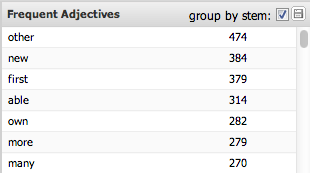
\includegraphics[width=0.5\textwidth]{fig/rex/02.png}
\caption{The most frequent adjectives overall in the literacy autobiographies \label{fig:rex02}}
\end{figure}

Faced with unexpected discoveries in every part of speech, Ganding decided to explore the adjectives (Figure \ref{fig:rex02}). The top three adjectives were not surprising - other (474), first (379), and new (384).  However,  ``able'' (314) and ``own'' (282) were words that he did not expect to be used frequently.

Ganding now wanted to understand the unexpectedly high frequencies of `able'' and ``own''. Our tool made this exploration easier. Instead of having to open a new window and type new search queries, clicking on the words themselves opened up Word Menus (Figure \ref{fig:rex03}) which allowed him to create word trees centered on those words (Figure \ref{fig:rex04}).  Word Trees \cite{wattenberg_word_2008} are an interactive visualizations that allow a user to explore the contexts in which a word is used. They group together common left- and right-contexts into a tree that gets finer and finer as the context get longer, terminating in individual sentences.  
\begin{figure}[h!]
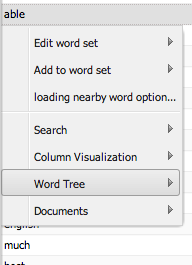
\includegraphics[width=0.2\textwidth]{fig/rex/03.png}
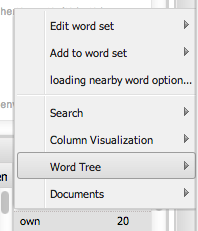
\includegraphics[width=0.2\textwidth]{fig/rex/03b.png}
\caption{Clicking on the `able' and `own' in the frequent adjectives list brings up a menu with the option to create Word Trees centered on those words in new panels. The results are shown in Figure \ref{fig:rex04} \label{fig:rex03}}
\end{figure}

\begin{figure*}[h!]
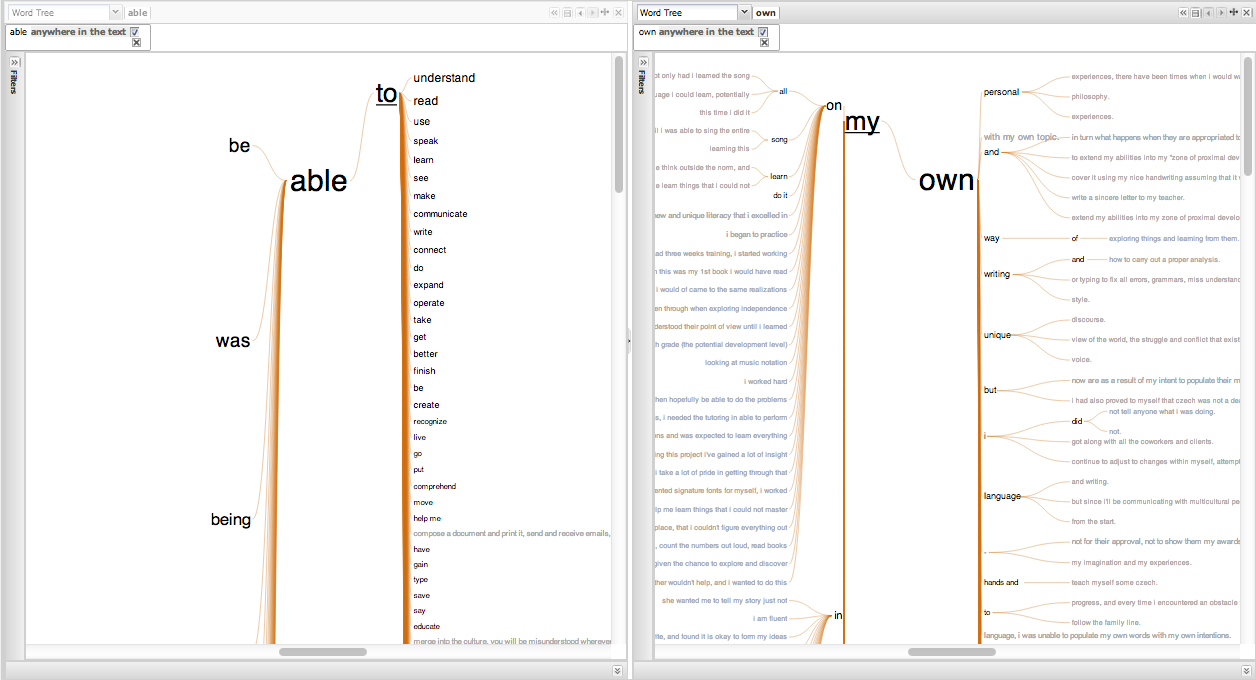
\includegraphics[width=\textwidth]{fig/rex/04.png}
\caption{ Two side-by-side Word Trees created from the word menu (with the bottom and side overview panels collapsed). On the left, the tree is centered on `able' and filtered to `able to', and on the right, the tree is centered on  `own' and filtered to `my own' in new panels \label{fig:rex04}}
\end{figure*}

The word tree for able (Figure \ref{fig:rex04} left) revealed that the most common use of the adjective able was: \code{[form of the verb `to be'] + able + to [action verb]} with the most common ``abilities'' being literacy-related: read, understand, communicate, learn, speak, etc.  For ``own'' (Figure \ref{fig:rex04} right), the most common construction was: \code{[preposition] + my + own}.  He also used the word tree to zoom in and read the individual sentences.

As a result, Ganding came away with a new insight about his students:
\begin{quote}
Student writers articulate their experiences from some first encounter with the unfamiliar, followed by a process of being ``able" to act within that which is becoming less unfamiliar.  Moving into literacy requires these writers to develop their ``own" abilities as necessary to survive and prosper in that context.
\end{quote} 

\subsubsection{Writing proficiency at across courses}
The different courses Ganding taught had different emphases and were taken by students with differing amounts of college education. He was especially interested in differences in sentence construction, hypothesizing that more proficient students would use advanced structures more frequently. To initiate the analyses, he performed word searches on terms such as ``though", ``while", ``although", and ``however", which indicate a complex structure called a ``concessive''. He was expecting them to be increasingly frequent as he moved from English 1A, to English 201, to English 5, to Ed140.

The Word Frequencies visualization allowed Ganding to confirm his hypothesis. It shows how often terms occur across different metadata categories (and can shown the counts stacked or grouped, or normalized or raw). Ganding searched for multiple terms simultaneously, which created a comparative visualization (Figure \ref{fig:rex05}).

\begin{figure}[h!]
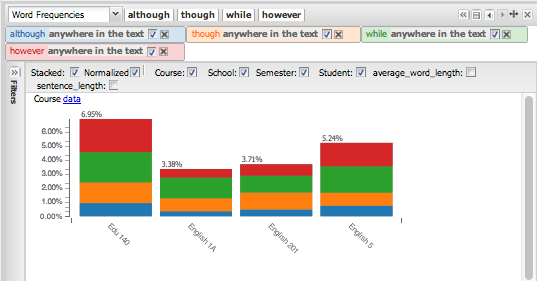
\includegraphics[width=0.5\textwidth]{fig/rex/05.png}
\caption{The normalized frequencies of different concessive words. Normalizing the counts adjusts for categories of unequal sizes, showing the percent of matching sentences in different categories instead of the counts. The words are `although' (blue), `though' (orange) `while' (green) and `however' (red). \label{fig:rex05}}
\end{figure}

The increasing frequencies across the course levels confirmed his hunch that as students become more experienced and comfortable with the written word, they used more complex sentence structures more frequently. 

\subsection{U.S. Perceptions of China and Japan}
[FirstName] Fan is a [scholar] at [university's] English department. Fan's research explores how US literature has responded to the rise of China since it began liberalizing its economy in the late 1970s.  His arguments rest on a set of historical observations about the rise of China  broadly accepted by historians and cultural historians: 
\begin{enumerate}
\item From the 1970s to the Tiananmen crackdown in 1989, US observers paid more attention to Japan than China. During this period, China didn't have much more than a strategic, Cold War relevance. 
\item With the onset of the 1990s, attention shifts from Japan to China. Japan entered its first ``Lost Decade'' of economic stagnation, and China, meanwhile, began deepening its economic relations with the US.
\item After China's accession to the World Trade Organization in 2001, US-China bilateral relationship becomes increasingly important to global economics and politics.
\item After 2001, there is an increasing sense that the US's time as the post-socialist era's last remaining superpower are numbered, and that China will replace it.
\end{enumerate}
Literary scholars typically allow their claims to rest on observations made by field experts like historians and sociologists, or on their own inductive reasoning. Fan, however, sought to supply these observations with as much empirical evidence as possible, as well as to verify them.

To generate this evidence, Fan collected New York Times editorials from  the Lexis/Nexis database, from 1980 to 2012. Using Lexis/Nexis's metadata, Fan limited the corpus of New York Times editorials to those with subjects ``China" or ``Japan." This resulted in a set of of 5,715 articles which were then imported to our tool.

\subsubsection{1970s through early-1990s: The China Card}
Fan verified his first claim using sliding interactions provided by the word menu and view switcher . His investigation began with an exploration of the ``grammatical neighborhood'' around `China'.

\begin{figure*}[h!]
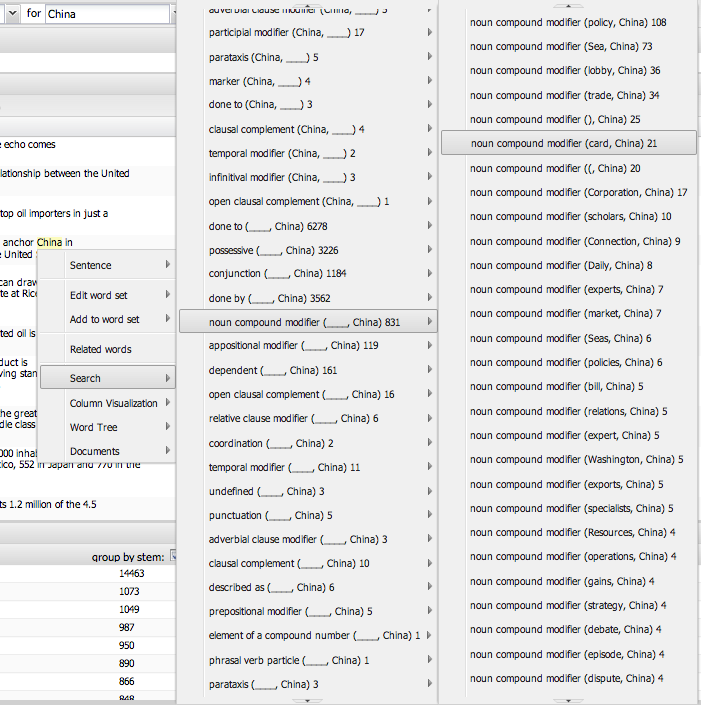
\includegraphics[width=\textwidth]{fig/chris/01.png}
\caption{The word menu for China allows a user to explore all the grammatical relationships in which ``China'' participates. The noun-compound relationship ``China card'' stood out to Fan. \label{fig:chris01}}
\end{figure*}

\begin{figure}[h!]
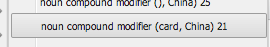
\includegraphics[width=0.3\textwidth]{fig/chris/01b.png}
\caption{ The menu option revealing that ``China card'' occurred 21 times over Fan's editorials. Clicking on it opens up the list of sentences containing ``China card''  \label{fig:chris01b}}
\end{figure}

As Figure \ref{fig:chris01} shows, clicking on the word ``China'' opens up a menu with search options. These options act as quick previews of different grammatically-related slices: they show the frequencies with which ``China'' occurs in different grammatical constructions with different words.  For Fan, the noun compound relationship yielded a surprise: an odd construction, ``China card,'' appeared 21 times.



Our tool allowed him to explore this this distinctive usage immediately. By selecting that very menu item (Figure \ref{fig:chris01b}), he was able to get a list of matching sentence. When Fan read those sentences, an interpretation suggested itself:
\begin{quote}[Reading] the sentence search results reveals that phrase is used to refer to the China's strategic value in Cold War geopolitics. Of the four post-2000 instances, only one uses the phrase to describe a contemporary political situation; the others use it to describe Cold War politics. Reducing the vastness of China to a disposable ``card,'' indicates a degree of US self-confidence, not to mention condescension, that disappears after 1989.\end{quote}
By sliding to a different view of the same data, he was able to verify the temporal claim. Using the drop-down menu at the top left of the panel (described earlier in Figure \ref{fig:chris03}) he selected a different view, Word Frequencies. This kept the slice the same (the sentences containing ``China card''), but opened up the word frequencies view alongside the list of search results.  Because the ``year'' metadata was attached to each article, this view displayed a graph of how frequent  sentences containing ``China Card'' were over time (Figure \ref{fig:chris02}). 

\begin{figure}[h!]
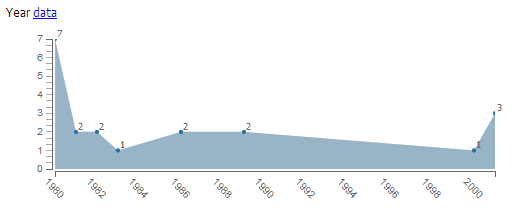
\includegraphics[width=0.5\textwidth]{fig/chris/02.png}
\caption{ The number of sentences matching ``China card'' over time. \label{fig:chris02}}
\end{figure}
This graph showed him that the cold war phrase, ``China card'' was used up until 1989, but rarely ever after that (he had already accounted for the later ones by looking at the sentences individually). This confirmed his claim that, up until the early 90's, china had a Cold-war strategic significance to the U.S. that later dissipated.

\section {Related Work}

\section{Discussion and Future Work}

\section{Acknowledgements}
We sincerely thank [Firstname Lastname, Firstname Lastname, and Firstname Lastname] for helpful comments on a Case Study not described in this paper. We are also grateful to [Firstname Lastname] for his helpful advice and thought-provoking discussions throughout.

This work is supported by NEH grant HK-50011-12.

\bibliographystyle{abbrv}
\bibliography{papers} 
  
\end{document}


